\documentclass[9pt]{article}

\newcommand{\nachr}{nAChR}
\newcommand{\plgic}{pLGIC}
\newcommand{\xo}{\textit{Xenopus} oocytes}
\usepackage{amsmath}
\usepackage{amssymb}
\usepackage{graphicx}
\usepackage{epstopdf}
\usepackage{inputenc}
\usepackage{geometry} 
\usepackage{adjustbox}
%  \usepackage[
%    backend=bibtex,
%    style=numeric,
%  ]{biblatex}
\usepackage[backend=bibtex]{biblatex}
\addbibresource{Paper_Bibs.bib} 

\title{Title of primary manuscript: supplemental document}

\begin{document}

\begin{titlepage}
   \begin{center}
      \huge\textbf{SUPPLEMENTARY MATERIAL}\\
      \LARGE{Spontaneous Lipid Binding to the Nicotinic Acetylcholine Receptor in a Native Membrane}\\
      
      
      Liam Sharp, Grace Brannigan
   \end{center}
   \vspace*{\stretch{2.0}}
   
\end{titlepage}

\renewcommand{\thefigure}{SI 1}
\begin{figure*}[!h]
	\center
	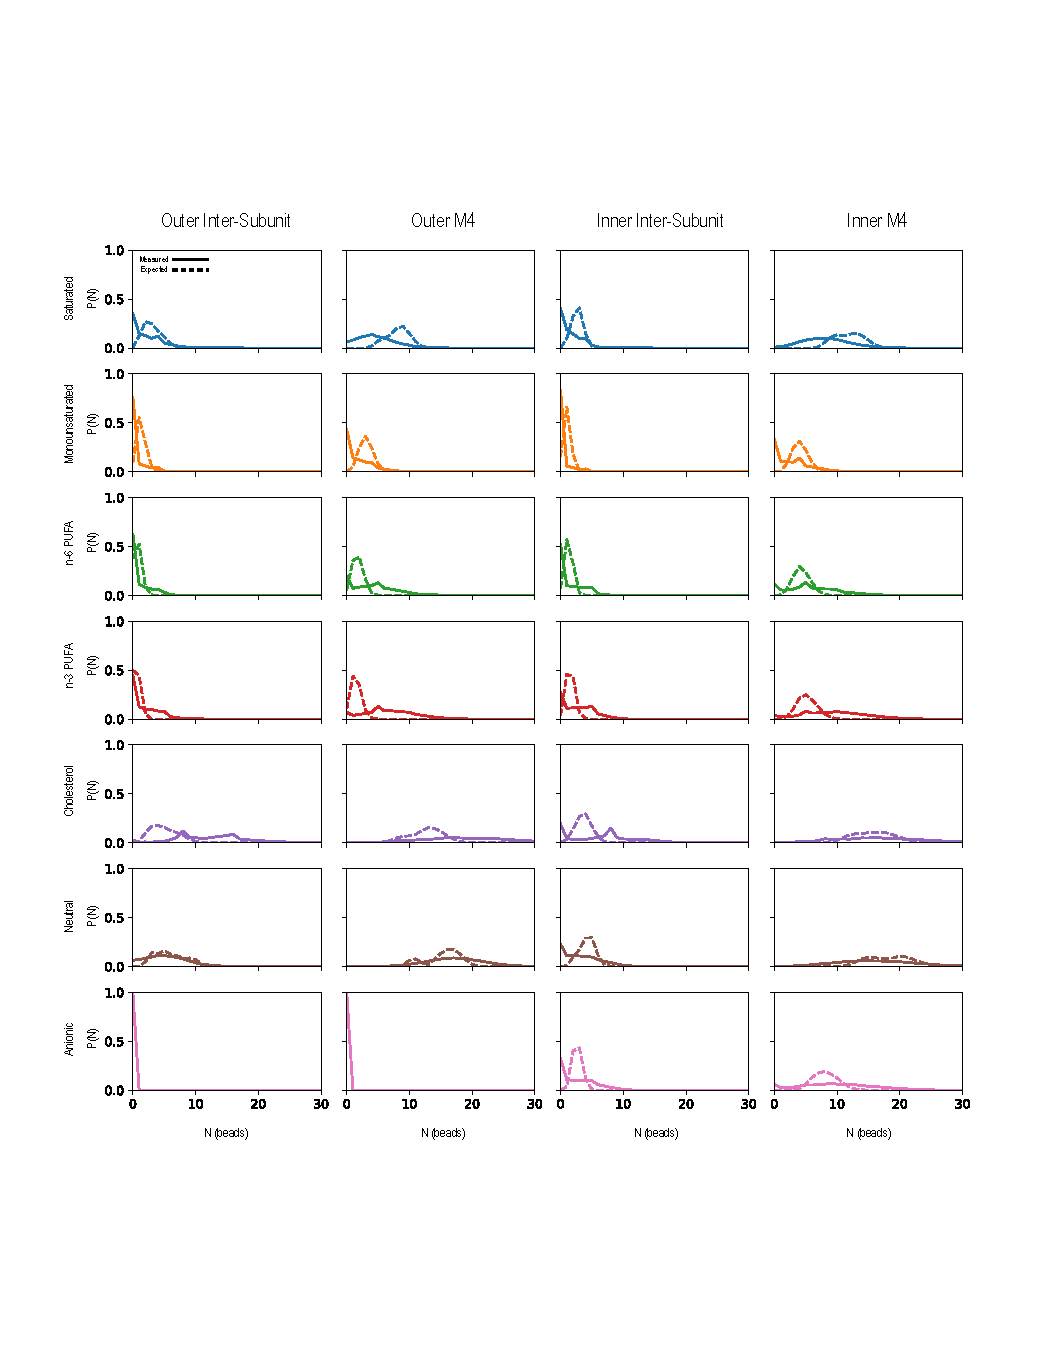
\includegraphics[width=\linewidth]{Bead_Distributions.pdf}
	\caption{Probability distributions of acyl-chain saturations, including cholesterol, and head group charge. Solid lines represent $P_{site}$, the probability of a given number of beads found at occupancy site, averaged over both the course of the simulation and subunit sites. Dashed lines represent  $P_{bulk}$, the probability of a given number of beads in the bulk averaged over time. Bulk areas are square regions of equal area to occupancy sites.}
	\label{fig:lipidDist}
\end{figure*}

\renewcommand{\thetable}{SI 1}
\begin{table}
    \caption{Lipid ratios used for neuronal simulations grouped by head group.}
    \label{tab:rats}
    \centering

\begin{tabular}{|c||c|cc|}

\hline
Head Group & Lipids & Outer (\%) &{Inner (\%)} \\ \hline\hline
{}&CHOL                         & 44.3     & 40.67                         \\
\hline
PC &{} &30.5&15\\ \hline
{} &DPPC                         & 6.7      & 3.3                           \\
{} &DOPC                         & 2.8      & 1.4                           \\
{} &POPC                         & 11     & 5.4                         \\
{} &PFPC                         & 0.7      & 0.4                           \\
{} &PAPC                         & 5.9      & 2.9                           \\
{} &PUPC                         & 2.1      & 1.0                           \\
{} &OIPC                         & 0.7      & 0.4                           \\
{} &OUPC                         & 0.5      & 0.3                           \\
\hline
\hline
PE &{} &13.8&23.4\\ \hline
{} &POPE                         & 1.6      & 2.7                           \\
{} &PAPE                         & 4      & 6.7                           \\
{} &PUPE                         & 6.3      & 10.7                          \\
{} &OIPE                         & 0.2      & 0.3                           \\
{} &OAPE                         & 0.9      & 1.5                           \\
{} &OUPE                         & 0.9      & 1.5                          \\
\hline
\hline
SM &{} &11.3&2.5\\ \hline
{} &DPSM                         & 7.4      & 1.7                           \\
{} &PBSM                         & 1.4      & 0.3                           \\
{} &POSM                         & 0.9      & 0.2                           \\
{} &PNSM                         & 1.7     & 0.4                           \\
\hline
\hline
PS &{} &0.0&10.8\\ \hline
{} &DPPS                         & 0.0      & 0.5                           \\
{} &POPS                         & 0.0      & 2.7                           \\
{} &PAPS                         & 0.0      & 3.0                           \\
{} &PUPS                         & 0.0      & 3.8   			\\      
{} &OUPS                         & 0.0      & 0.8                           \\
\hline       
\hline          
PA &{} &0.0&0.4\\ \hline
{} &POPA                         & 0.0      & 0.1                          \\
{} &PAPA                         & 0.0      & 0.3                           \\
\hline
\hline
PI &{} &0.0&2.3\\ \hline
{} &POPI                         & 0.0      & 1.4                         \\
{} &PIPI                         & 0.0      & 0.6                           \\
{} &PAPI                         & 0.0      & 1.4                           \\
{} &PUPI                         & 0.0      & 2.3                           \\
\hline
\hline
PIPS &{} &0.0&1.5\\ \hline
{} &POP1                         & 0.0      & 0.2                           \\
{} &PAP1                         & 0.0      & 0.3                           \\
{} &POP2                         & 0.0      & 0.2                           \\
{} &PAP2                         & 0.0      & 0.3                           \\
{} &POP3                         & 0.0      & 0.2                           \\
{} &PAP3                         & 0.0      & 0.3                           \\
\hline
\end{tabular}
\end{table}

\renewcommand{\thefigure}{SI 2}

\begin{figure}
	\center
	\includegraphics[width=2in]{Anonic_AA.pdf}
	%\includegraphics[width=2in]{../Figures/Anonic_AA.pdf}
	\caption{Charged amino acids in or near the TMD of two \plgic s and corresponding anionic enrichment. a) Structure of the TMD viewed from the extracellular side looking at the membrane, of \nachr~(top)\cite{Unwin2005} and ELIC\cite{Pan2012} (bottom). \nachr~ is colored as in Figure 1, ELIC is cyan. Basic amino acids are colored in blue while acidic amino acids are colored in red for both structures. b) Anionic polar density enrichment observed in ELIC, derived from \cite{Tong2019}. Grey circles represent center of mass of alpha-helices, red circles represent center of mass of alpha-helices with basic amino acids. }
	\label{fig:aaa}
\end{figure}
\renewcommand{\thetable}{SI 2}

\begin{table*}
    \caption{Affinities broken down by headgroup and acyl chain to reveal cross-correlation. }
    \centering
  \resizebox{\textwidth}{!}{  \begin{tabular}{|l||cc|cc|}
        
        \hline
        {} &  Outer Inter Sites&  Outer M4 Sites&  Inner Inter Sites&  Inner M4 Sites\\
        {} & $\Delta G$ (kcal/mol) & $\Delta G$ (kcal/mol) & $\Delta G$ (kcal/mol) & $\Delta G$ (kcal/mol) \\
        \hline
        
        CHOL &-1.5 $\pm$0.4& -0.8$\pm$0.3&    -0.6$\pm$0.3& -0.1$\pm$0.2\\
        Sat   &  0.7 $\pm$0.3	&  1.3 $\pm$0.2&     1.0 $\pm$	0.2&  1.1 $\pm$0.2 \\
        Mono   &    1.2 $\pm$0.2&  0.8$\pm$	0.2&     1.4 $\pm$0.1&  0.7 $\pm$0.2\\
        n-6   &         0.6 $\pm$0.2& -0.5 $\pm$0.1&0.3 $\pm$0.2& -0.3 $\pm$0.2\\
        n-3   &       -0.0 $\pm$0.4& -1.3 $\pm$0.3&    -0.2$0.2\pm$ & -0.9$\pm$0.2\\
        \hline
        Neutral &     0.4 $\pm$0.3& -0.4$\pm$0.2 &     0.5 $\pm$0.2&  0.5$\pm$0.2 \\
        Anionic &     2.4 $\pm$0.4&  2.4 $\pm$0.4&     0.3 $\pm$0.2& -0.3 $\pm$0.1\\
	\hline
        \hline
        Sat Neutral &  0.8 $\pm$0.2&  1.3 $\pm$0.1&     1.1$\pm$0.1 &  1.1 $\pm$0.2\\
        Mono Neutral & 1.2$\pm$0.2&  0.9 $\pm$0.1&     1.6 $\pm$0.2&  0.6 $\pm$0.1\\
        n-6 Neutral &  0.7 $\pm$0.2& -0.5 $\pm$0.2&     1.0 $\pm$0.2&  0.0 $\pm$0.1\\
        n-3 Neutral &  0.1 $\pm$0.3& -1.2$\pm$0.3& 0.2 $\pm$0.1& -0.4 $\pm$0.1\\
        \hline
        \hline
        Sat Anionic &&& 1.3$\pm$0.2 &  0.4$\pm$0.1\\
        Mono Anionic &&& 2.5 $\pm$0.4&  1.2 $\pm$0.4\\
        n-6 Anionic &&&1.1 $\pm$0.3&  0.3$\pm$0.2\\
        n-3 Anionic && &0.8 $\pm$0.3&  0.1 $\pm$0.2\\
        \hline

        \hline
        
    \end{tabular}}
    \label{tab:dGTab}
\end{table*}


\renewcommand{\thetable}{SI 3.1}
\begin{table}
    \caption{{Complete listing of affinities for intersubunit sites in the outer leaflet.}}
    \centering
    \tiny

\resizebox{\textwidth}{!}{ \begin{tabular}{| c || ccccc |}
\hline
    Lipids     & Outer $\alpha_{\gamma}-\beta$  & Outer $\beta-\delta$ & Outer $\delta-\alpha_{\delta}$  & Outer $\alpha_{\delta}-\gamma$  & Outer $\gamma-\alpha_{\gamma}$  \\
        \hline
        & ($\Delta G$ (kcal/mol)) & ($\Delta G$ (kcal/mol)) & ($\Delta G$ (kcal/mol)) & ($\Delta G$ (kcal/mol)) & ($\Delta G$ (kcal/mol)) \\
Lipid Species &&&&&\\
CHOL    &-0.9&-1.4&-1.5&-1.6&-2.0\\
DOPC    &3.5&3.4&2.2&2.8&2.3\\
DPPC    &3.3&2.1&2.3&1.4&2.0\\
DPPS    &4.1&4.1&4.2&3.9&4.2 \\
DPSM    &2.1&2.7&2.3&1.2&2.1\\
OAPE    &1.9&2.5&1.9&1.4&1.9\\
OIPC    &3.0&2.9&2.4&4.0&2.6\\
OIPE    &2.4&4.0&3.5&3.8&2.4\\
OUPC    &2.0&2.2&1.9&1.7&2.9\\
OUPE    &0.9&1.0&1.4&2.0&1.7\\
%OUPS    &3.7&3.8&3.5&3.7&3.4\\
%PAP1&4.6&4.2&4.3&4.4&4.4\\
%PAP2&4.9&4.6&4.9&5.3&3.9\\
%PAP3&4.2&4.1&4.2&4.0&4.3\\
%PAPA    &4.9&4.0&4.2&4.3&4.4\\
PAPC    &0.6&0.9&1.0&1.1&1.2\\
PAPE    &1.1&1.2&1.1&1.4&1.2\\
%%PAPI    &3.2&3.3&3.6&3.3&3.3\\
%PAPS    &3.1&3.0&3.0&3.0&3.1\\
PBSM    &4.9&4.9&3.4&4.4&3.1\\
PFPC    &1.9&1.3&2.4&3.1&3.3\\
%PIPI    &4.0&4.6&3.9&4.6&4.2\\
PNSM    &3.2&4.9&2.5&4.3&2.7\\
%%POP1&4.3&4.6&5.3&4.3&4.4\\
%POP2&4.6&5.3&            &4.9&   \\         
%POP3&4.3&4.6&5.3&            &4.9\\
%POPA    &            &5.3&            &            & \\           
POPC    &2.2&1.8&1.7&2.0&1.6\\
POPE    &2.8&2.6&2.4&3.0&2.6\\
%POPI    &3.6&3.4&3.6&3.6&3.5\\
%POPS    &3.3&3.2&3.1&3.1&3.0\\
POSM    &3.3&2.6&3.8&2.9&3.4\\
PUPC    &1.4&1.5&1.9&1.0&1.9\\
PUPE    &0.0&0.3&0.1&-0.5&0.2\\
%PUPI    &3.2&3.2&3.0&3.1&3.1\\
%PUPS    &2.8&2.8&2.8&2.9&2.8\\
\hline
Head Groups 
PC      &0.9&0.4&1.0&0.7&1.1\\
PE      &-0.4&-0.3&-0.2&-0.3&0.4\\
SM      &1.9&2.5&2.2&1.2&2.0\\
%PS      &2.5&2.6&2.5&2.6&2.5\\
%PA      &4.9&3.9&4.2&4.3&4.4\\
%PI      &2.7&2.8&2.8&2.9&2.7\\
%PIP1&4.3&4.1&4.2&4.0&4.2\\
%PIP2&4.3&4.4&5.3&4.9&3.9\\
%PIP3&4.0&4.0&4.2&4.2&4.2\\
\hline
Acyl-Chain Saturation 
Sat      &1.0&0.6&0.9&0.5&0.7\\
Monounsat      &1.1&1.1&1.1&1.3&1.4\\
n-6&0.4&0.5&0.8&0.7&0.7\\
n-3&-0.2&-0.2&0.0&-0.1&0.5\\
\hline
Head Group Charge&&&&&\\
Neutral &0.7&-0.1&0.7&0.2&0.5\\
%Anionic &2.4&2.4&2.4&2.4&2.4\\
\hline
Acyl-Chain Saturation by Charge 
Neutral Sat    &1.0&0.6&0.9&0.5&1.2\\
Neutral Monounsat    &1.1&1.2&1.1&1.3&1.4\\
Neutral n-6&0.4&0.5&0.8&0.7&1.1\\
Neutral n-3&-0.2&0.2&0.3&-0.1&0.5\\
\hline
%Anionic Sat     &2.5&2.5&2.5&2.5&2.4\\
%Anionic Monounsat    &3.0&3.0&3.1&3.1&2.8\\
%Anionic n-6&3.0&2.8&2.9&3.0&2.9\\
%Anionic n-3&2.7&2.8&2.8&2.8&2.7\\
%\hline
\end{tabular}}
\end{table}

\renewcommand{\thetable}{SI 3.2}
\begin{table}
    \caption{Complete listing of affinities for M4 sites in the outer leaflet.}
    \centering
    \tiny

\resizebox{\textwidth}{!}{\begin{tabular}{| c || ccccc |}
\hline
     Lipids     & Outer $\alpha_{\gamma}$   & Outer $\beta$   & Outer $\delta$    & Outer $\alpha_{\delta}$   & Outer $\gamma$   \\
        \hline
        & ($\Delta G$ (kcal/mol)) & ($\Delta G$ (kcal/mol)) & ($\Delta G$ (kcal/mol)) & ($\Delta G$ (kcal/mol)) & ($\Delta G$ (kcal/mol)) \\
Lipid Species &&&&&\\
CHOL    &-1.0&-1.3&-0.8&-0.8&-0.2\\
DOPC    &1.8&2.1&1.5&1.5&1.9\\
DPPC    &1.3&2.0&1.7&2.2&1.8\\
%DPPS    &3.5&3.8&3.7&3.7&3.6\\
DPSM    &1.6&1.5&1.7&1.7&2.0\\
OAPE    &1.5&1.3&1.3&0.9&1.1\\
OIPC    &2.2&1.8&2.8&2.1&2.2\\
OIPE    &2.0&2.2&3.1&2.6&2.8\\
OUPC    &1.7&1.5&1.5&1.5&1.3\\
OUPE    &0.6&0.8&0.8&0.9&0.9\\
%OUPS    &3.2&3.3&3.6&3.3&3.4\\
%PAP1&4.0&4.3&3.9&4.3&4.0\\
%PAP2&4.2&4.4&4.6&4.6&3.9\\
%PAP3&3.9&4.1&3.9&3.6&3.9\\
%PAPA    &4.4&4.4&3.9&3.9&4.4\\
PAPC    &0.2&0.3&0.5&0.3&0.2\\
PAPE    &0.4&0.3&0.1&0.4&0.4\\
%PAPI    &3.0&3.0&3.4&3.1&3.1\\
%PAPS    &2.9&3.0&2.8&2.8&2.9\\
PBSM    &2.7&3.0&3.5&2.7&2.9\\
PFPC    &2.0&1.3&1.9&1.8&1.7\\
%PIPI    &3.5&3.7&3.5&3.7&4.4\\
PNSM    &2.3&2.3&2.5&2.5&2.6\\
%POP1&4.3&4.0&4.9&5.3&4.1\\
%POP2&4.9&4.9&5.3&5.3&4.2\\
%POP3&4.2&4.3&4.6&4.6&4.9\\
%POPA    &5.3&4.9&4.9&4.9&5.3\\
POPC    &1.1&1.4&1.5&1.4&1.7\\
POPE    &1.9&1.9&1.7&1.7&2.3\\
%POPI    &3.3&3.3&3.1&3.3&3.1\\
%POPS    &2.8&3.0&2.9&2.8&2.7\\
POSM    &2.7&2.8&2.8&2.9&2.9\\
PUPC    &0.5&0.8&1.0&0.8&0.5\\
PUPE    &-0.3&-0.6&-0.6&-1.0&-0.9\\
%PUPI    &2.8&3.0&2.9&2.9&2.8\\
%PUPS    &2.6&2.7&2.6&2.7&2.7\\
\hline
Head Groups &&&&&\\
PC      &0.3&0.2&0.8&0.8&0.3\\
PE      &-0.7&-1.0&-1.3&-1.3&-1.2\\
SM      &1.5&1.6&1.8&1.8&1.9\\
%PS      &2.4&2.5&2.4&2.4&2.4\\
%PA      &4.3&4.2&3.8&3.8&4.3\\
%PI      &2.5&2.6&2.6&2.6&2.6\\ $\Delta G$ ($\Delta G$ (kcal/mol))
%PIP1&3.8&3.9&3.9&4.6&3.7\\
%PIP2&4.4&4.3&4.9&4.9&3.9\\
%PIP3&3.9&3.9&3.9&3.6&3.8\\
\hline
Acyl-Chain Saturation &&&&&\\
Sat      &1.0&1.0&1.3&1.9&1.4\\
Monounsat      &0.8&0.7&0.7&0.7&1.1\\
n-6&-0.4&-0.6&-0.3&-0.5&-0.4\\
n-3&-1.1&-1.2&-1.0&-1.3&-1.8\\
\hline
Head Group Charge &&&&&\\
Neutral &-0.2&-0.9&0.0&0.0&-0.7\\
%Anionic &2.4&2.4&2.4&2.4&2.4\\
\hline
Acyl-Chain Saturation by Charge 
Neutral Sat    &1.0&1.0&1.3&2.0&1.4\\
Neutral Monounsat    &0.8&0.7&0.7&1.2&1.1\\
Neutral n-6&-0.4&-0.6&-0.3&-0.5&-0.4\\
Neutral n-3&-0.8&-1.2&-1.0&-1.3&-1.8\\
\hline
%Anionic Sat     &2.4&2.5&2.4&2.4&2.4\\
%Anionic Monounsat    &2.7&2.8&2.8&2.7&2.7\\
%Anionic n-6&2.7&2.7&2.7&2.7&2.8\\
%Anionic n-3&2.5&2.6&2.6&2.6&2.6\\
\end{tabular}}
\end{table}

\renewcommand{\thetable}{SI 3.3}
\begin{table}
    \caption{Complete listing of affinities for intersubunit sites in the inner leaflet.}
    \centering
    \tiny

\resizebox{\textwidth}{!}{\begin{tabular}{| c || ccccc |}
\hline
   Lipids     & Inner $\alpha_{\gamma}-\beta$  & Inner $\beta-\delta$  & Inner $\delta-\alpha_{\delta}$ & Inner $\alpha_{\delta}-\gamma$  & Inner $\gamma-\alpha_{\gamma}$  \\
        \hline
        & ($\Delta G$ (kcal/mol)) & ($\Delta G$ (kcal/mol)) & ($\Delta G$ (kcal/mol)) & ($\Delta G$ (kcal/mol)) & ($\Delta G$ (kcal/mol)) \\
Lipid Species &&&&&\\
CHOL    &-0.4&-0.4&-1.1&0.3&-1.2\\
DOPC    &2.4&3.1&2.9&2.6&2.9\\
DPPC    &1.9&2.7&2.1&2.3&2.1\\
DPPS    &4.4&4.2&3.5&4.9&5.3\\
DPSM    &2.5&1.7&2.1&2.6&2.5\\
OAPE    &2.3&2.5&1.9&1.9&3.1\\
OIPC    &3.1&2.9&3.8&3.0&3.4\\
OIPE    &4.9&3.3&3.5&3.8&3.3\\
OUPC    &3.1&3.2&2.3&2.7&2.1\\
OUPE    &2.4&1.4&1.5&1.8&1.7\\
OUPS    &2.4&2.8&1.5&2.2&2.1\\
PAP1&1.4&3.3&1.5&1.6&2.9\\
PAP2&1.9&3.9&            &1.1&2.1\\
PAP3&2.7&1.7&3.2&1.6&2.0\\
PAPA    &3.9&2.4&2.7&3.1&3.2\\
PAPC    &1.7&1.7&1.7&1.6&1.9\\
PAPE    &0.9&1.5&1.1&1.4&1.2\\
PAPI    &1.7&1.7&1.9&1.6&1.4\\
PAPS    &1.5&2.2&1.8&1.7&1.7\\
PBSM    &3.2&3.5&3.5&3.8&3.5\\
PFPC    &2.2&2.6&2.9&2.6&3.6\\
PIPI    &3.6&2.9&1.8&3.3&2.4\\
PNSM    &3.0&2.8&2.8&3.6&3.2\\
POP1&5.3&            &3.2&3.3&4.6\\
POP2&3.5&3.5&3.5&3.4&            \\
POP3&3.2&4.4&            &3.4&            \\
POPA    &            &            &5.3&5.3&       \\     
POPC    &2.4&1.7&2.0&2.0&1.8\\
POPE    &2.7&3.0&2.6&3.4&2.4\\
POPI    &2.4&2.9&2.5&2.4&2.3\\
POPS    &2.7&3.0&1.7&3.8&2.8\\
POSM    &3.9&4.1&2.7&4.3&3.4\\
PUPC    &2.0&1.7&1.7&2.1&2.0\\
PUPE    &0.1&0.2&0.4&0.5&0.4\\
PUPI    &1.0&1.0&1.4&1.1&0.7\\
PUPS    &1.2&1.7&1.0&1.5&1.6\\
\hline
Head Groups 
PC      &1.1&1.0&1.1&1.2&1.5\\
PE      &-0.1&0.3&0.3&0.4&0.6\\
SM      &2.4&1.7&1.9&2.6&2.5\\
PS      &0.8&1.4&0.5&1.1&1.4\\
PA      &3.7&2.5&2.6&3.1&3.3\\
PI      &0.9&0.9&1.0&0.9&1.0\\
PIP1&1.5&3.6&1.6&2.0&3.3\\
PIP2&2.1&4.0&4.1&1.3&2.4\\
PIP3&3.3&2.2&3.6&1.8&2.3\\
\hline
Acyl-Chain Saturation 
Sat      &0.7&1.1&0.9&1.1&1.3\\
Monounsat      &1.4&1.5&0.9&1.4&1.6\\
n-6&0.1&0.6&0.3&0.0&0.7\\
n-3&-0.3&0.0&-0.3&-0.2&0.1\\
\hline
Head Group Charge 
Neutral &0.4&0.7&0.5&0.5&0.5\\
Anionic &0.1&0.8&0.1&0.1&0.4\\
\hline
Acyl-Chain Saturation by Charge 
Neutral Sat    &1.0&1.1&1.1&1.3&1.3\\
Neutral Monounsat    &1.7&1.6&1.5&1.6&1.4\\
Neutral n-6&0.7&1.2&0.8&1.0&1.4\\
Neutral n-3&0.0&0.0&0.1&0.3&0.6\\
\hline
Anionic Sat     &1.0&1.6&1.1&1.3&1.3\\
Anionic Monounsat    &2.4&3.0&1.6&3.0&2.4\\
Anionic n-6&0.9&1.6&1.1&0.6&1.1\\
Anionic n-3&0.7&1.1&0.6&0.9&0.8\\
\hline
\end{tabular}}
\end{table}

\renewcommand{\thetable}{SI 3.4}
\begin{table}
    \caption{Complete listing of affinities for M4 sites in the inner leaflet.}
        \tiny
	\centering

\resizebox{\textwidth}{!}{\begin{tabular}{| c || ccccc |}
\hline	
     Lipids     & Inner $\alpha_{\gamma}$    & Inner$\beta$   & Inner $\delta$    & Inner $\alpha_{\delta}$    & Inner $\gamma$   \\
        \hline
        & ($\Delta G$ (kcal/mol)) & ($\Delta G$ (kcal/mol)) & ($\Delta G$ (kcal/mol)) & ($\Delta G$ (kcal/mol)) & ($\Delta G$ (kcal/mol)) \\ \hline 
Lipid Species &&&&&\\
CHOL    &-0.3&0.2&-0.4&-0.3&0.3        \\
DOPC    &1.6&1.4&1.8&1.5&1.6        \\
DPPC    &1.1&1.1&1.4&1.2&1.3        \\
DPPS    &2.2&2.6&2.9&2.6&3.1        \\
DPSM    &1.6&1.3&1.6&1.3&1.6        \\
OAPE    &1.4&1.3&1.5&1.2&1.4        \\
OIPC    &2.1&2.0&2.2&2.0&1.9        \\
OIPE    &2.2&2.8&2.7&2.1&2.4        \\
OUPC    &2.2&2.3&2.6&2.0&1.6        \\
OUPE    &1.2&1.0&1.0&0.9&0.8        \\
OUPS    &1.5&2.0&1.6&1.5&1.6        \\
PAP1&2.6&1.7&2.4&1.9&1.3        \\
PAP2&2.7&1.7&2.8&2.4&1.1        \\
PAP3&2.0&1.9&1.3&2.3&1.1        \\
PAPA    &2.6&1.9&2.4&2.6&2.0        \\
PAPC    &0.8&0.8&0.9&0.7&0.8        \\
PAPE    &0.4&0.4&0.5&0.3&0.4        \\
PAPI    &1.2&1.1&1.0&1.2&1.1        \\
PAPS    &0.8&0.9&1.1&1.0&0.7        \\
PBSM    &2.2&2.1&2.3&2.5&2.5        \\
PFPC    &2.2&2.0&2.1&1.9&2.1        \\
PIPI    &2.3&2.1&2.3&1.8&2.7        \\
PNSM    &2.4&2.1&2.1&1.9&2.5        \\
POP1&3.6&3.5&2.9&3.0&2.6        \\
POP2&3.9&2.6&2.4&3.0&2.6        \\
POP3&2.9&2.9&2.9&3.3&2.2        \\
POPA    &3.1&3.2&3.8&3.1&3.4        \\
POPC    &0.9&1.0&0.9&0.9&1.1        \\
POPE    &1.3&1.3&1.6&1.4&1.6        \\
POPI    &1.5&1.6&1.7&1.3&1.7        \\
POPS    &1.6&1.6&1.5&1.5&1.8        \\
POSM    &2.5&2.7&2.9&2.8&2.6        \\
PUPC    &1.5&1.2&1.5&1.1&1.0        \\
PUPE    &-0.1&-0.4&-0.1&-0.1&-0.3       \\
PUPI    &0.9&0.4&0.4&0.9&0.3        \\
PUPS    &0.9&0.7&0.5&0.8&0.7        \\
\hline
Head Groups &&&&&\\
PC      &0.6&0.7&0.8&0.7&0.6        \\
PE      &0.0&-0.2&-0.3&-0.1&-0.1       \\
SM      &1.4&1.4&1.4&1.1&1.6        \\
PS      &0.3&0.5&0.3&0.5&0.3        \\
PA      &2.5&1.8&2.4&2.5&2.0        \\
PI      &0.4&0.2&0.1&0.4&0.1        \\
PIP1&2.7&1.8&2.3&2.1&1.4        \\
PIP2&2.8&1.7&2.3&2.4&1.2        \\
PIP3&2.0&2.1&1.4&2.3&1.2        \\
\hline
Acyl-Chain Saturation &&&&&\\
Sat      &0.9&1.2&0.8&1.4&1.2        \\
Monounsat      &0.4&0.8&0.5&0.8&0.9        \\
n-6&-0.1&-0.4&-0.3&-0.1&-0.6       \\
n-3&-0.5&-1.0&-1.0&-0.5&-1.2       \\
\hline
Head Group Charge  &&&&&\\
Neutral &0.3&0.4&0.3&0.6&0.5        \\
Anionic &0.0&-0.3&-0.4&0.2&-0.7      \\
\hline
Acyl-Chain Saturation by Charge &&&&&\\
Neutral Sat    &0.9&1.2&0.8&1.2&1.4        \\
Neutral Monounsat    &0.5&0.7&0.6&0.4&0.8        \\
Neutral n-6&0.0&0.1&0.1&-0.1&0.1        \\
Neutral n-3&-0.2&-0.6&-0.4&-0.4&-0.6       \\
Anionic Sat     &0.3&0.5&0.1&0.7&0.3        \\
Anionic Monounsat    &1.1&1.2&1.2&1.2&1.2        \\
Anionic n-6&0.5&0.2&0.5&0.5&-0.1       \\
Anionic n-3&0.5&0.0&0.0&0.3&-0.1       \\\hline
\end{tabular}}
\end{table}

\renewcommand{\thetable}{SI 4.1}
\begin{table}
    \caption{Table SI Parameters used for calculating density threshold affinitiesfor intersubunit sites in the outer leaflet. Angular and radial boundaries are used to define sites for a given total area. Accessible areas are as described in Methods \textit{Binding Site Definition and Occupancy Calculations}. Methods \textit{Calculation of Accessible Area}}
    \centering
\resizebox{\textwidth}{!}{ \begin{tabular}{| c || ccccc |}
\hline
   {}     & Outer $\alpha_{\gamma}-\beta$  & Outer $\beta-\delta$ & Outer $\delta-\alpha_{\delta}$  & Outer $\alpha_{\delta}-\gamma$  & Outer $\gamma-\alpha_{\gamma}$  \\ \hline
  Angular Boundaries &$1.13\geq\theta\leq1.63$ rad&$0.37\geq\theta\leq6.16$ rad&$4.9\geq\theta\leq5.4$ rad&$3.64\geq\theta\leq4.15$ rad&$2.38\geq\theta\leq2.89$ rad\\
 Radial Boundaries &$10<r\leq32$\AA&$10<r\leq32$\AA&$10<r\leq32$\AA&$10<r\leq32$\AA&$10<r\leq32$\AA\\
  Total Area &301.59\AA$^2$&361.91\AA$^2$&301.59\AA$^2$&301.59\AA$^2$&301.59\AA$^2$\\
  Accessible Area &104.40\AA$^2$&50.89\AA$^2$&63.80&81.20\AA$^2$&34.80\AA$^2$\\


  \hline

\end{tabular} }
\end{table}

\renewcommand{\thetable}{SI 4.2}
\begin{table}
    \caption{Table SI Parameters used for calculating density threshold affinities for M4 sites in the outer leaflet. Angular and radial boundaries are used to define sites for a given total area. Accessible areas are as described in Methods \textit{Binding Site Definition and Occupancy Calculations}. Methods \textit{Calculation of Accessible Area}}
    \centering
\resizebox{\linewidth}{!}{ \begin{tabular}{| c || ccccc |}
\hline
 {}     & Outer $\alpha_{\gamma}$   & Outer $\beta$   & Outer $\delta$    & Outer $\alpha_{\delta}$   & Outer $\gamma$  \\ 
 \hline
   Angular Boundaries &$1.76\geq\theta\leq2.26$ rad&$0.5\geq\theta\leq1$ rad&$5.52\geq\theta\leq6.03$ rad&$4.27\geq\theta\leq4.78$ rad&$3.02\geq\theta\leq3.52$ rad\\
   Radial Boundaries &$10<r\leq44$\AA&$10<r\leq44$\AA&$10<r\leq44$\AA&$10<r\leq44$\AA&$10<r\leq44$\AA\\
  Total Area &703.72\AA$^2$&703.72\AA$^2$&703.72\AA$^2$&703.72\AA$^2$&703.72\AA$^2$\\
  Accessible Area &173.14\AA$^2$&117.29\AA$^2$&184.31\AA$^2$&195.48\AA$^2$&161.97\AA$^2$\\


  \hline

\end{tabular} }
\end{table}

\renewcommand{\thetable}{SI 4.3}
\begin{table}
    \caption{Table SI Parameters used for calculating density threshold affinities for intersubunit sites in the inner leaflet. Angular and radial boundaries are used to define sites for a given total area. Accessible areas are as described in Methods \textit{Binding Site Definition and Occupancy Calculations}. Methods \textit{Calculation of Accessible Area}}
    \centering
\resizebox{\linewidth}{!}{ \begin{tabular}{| c || ccccc |}
\hline
   {}     & Inner $\alpha_{\gamma}-\beta$  & Inner $\beta-\delta$  & Inner $\delta-\alpha_{\delta}$ & Inner $\alpha_{\delta}-\gamma$  & Inner $\gamma-\alpha_{\gamma}$  \\
   \hline
   Angular Boundaries &$1.38\geq\theta\leq1.88$ rad&$0.13\geq\theta\leq0.62$ rad&$5.15\geq\theta\leq5.65$ rad&$3.77\geq\theta\leq4.27$ rad&$2.64\geq\theta\leq3.01$ rad\\
   Radial Boundaries &$10<r\leq32$\AA&$10<r\leq32$\AA&$10<r\leq32$\AA&$10<r\leq32$\AA&$10<r\leq32$\AA\\
  Total Area &301.59\AA$^2$&241.27\AA$^2$&301.59\AA$^2$&241.27\AA$^2$&241.27\AA$^2$\\
  Accessible Area &68.29\AA$^2$&74.68\AA$^2$&68.29\AA$^2$&63.19\AA$^2$&40.21\AA$^2$\\

  \hline

\end{tabular} }
\end{table}

\renewcommand{\thetable}{SI 4.4}
\begin{table}
    \caption{Table SI Parameters used for calculating density threshold affinities for M4 in the inner leaflet. Angular and radial boundaries are used to define sites for a given total area. Accessible areas are as described in Methods \textit{Binding Site Definition and Occupancy Calculations}. Methods \textit{Calculation of Accessible Area}}
    \centering
\resizebox{\linewidth}{!}{ \begin{tabular}{| c || ccccc |}
\hline
   {}     & Inner $\alpha_{\gamma}$    & Inner$\beta$   & Inner $\delta$    & Inner $\alpha_{\delta}$    & Inner $\gamma$\\   \hline
   Angular Boundaries &$2.01\geq\theta\leq2.51$ rad&$.75\geq\theta\leq1.26$ rad&$5.78\geq\theta\leq6.16$ rad&$4.4\geq\theta\leq5.03$ rad&$3.14\geq\theta\leq3.64$ rad\\
   Radial Boundaries &$10<r\leq44$\AA&$10<r\leq44$\AA&$10<r\leq44$\AA&$10<r\leq44$\AA&$10<r\leq44$\AA\\
  Total Area &703.72\AA$^2$&844.46\AA$^2$&703.72\AA$^2$&844.46\AA$^2$&844.46\AA$^2$\\
  Accessible Area &211.69\AA$^2$&273.88\AA$^2$&205.97\AA$^2$&302.41\AA$^2$&273.88\AA$^2$\\
  \hline

\end{tabular} }
\end{table}
\clearpage
\printbibliography
\end{document}